\textbf{This is an interactive problem}

In the vast kingdom of DataLand, the wise King Algorithmus has hidden a series of magical scrolls along a secret path. Each scroll contains a number, and the scrolls are arranged in strict order, with each successive scroll bearing a larger number than the last. The kingdom's scholars refer to this path as a \textit{singly linked list}, where each scroll not only holds a number but also points to the next scroll in the sequence.

You, the kingdom's chief seeker, have been tasked with finding the first scroll whose number is not less than a magical number $x$, which the king has entrusted to you. The challenge lies in the fact that the path is long, and you may only inspect a limited number of scrolls before the path vanishes into the mists of time.

\begin{center}
  \def \htmlPixelsInCm {45}  % pixels in 1 centimeter in HTML mode
  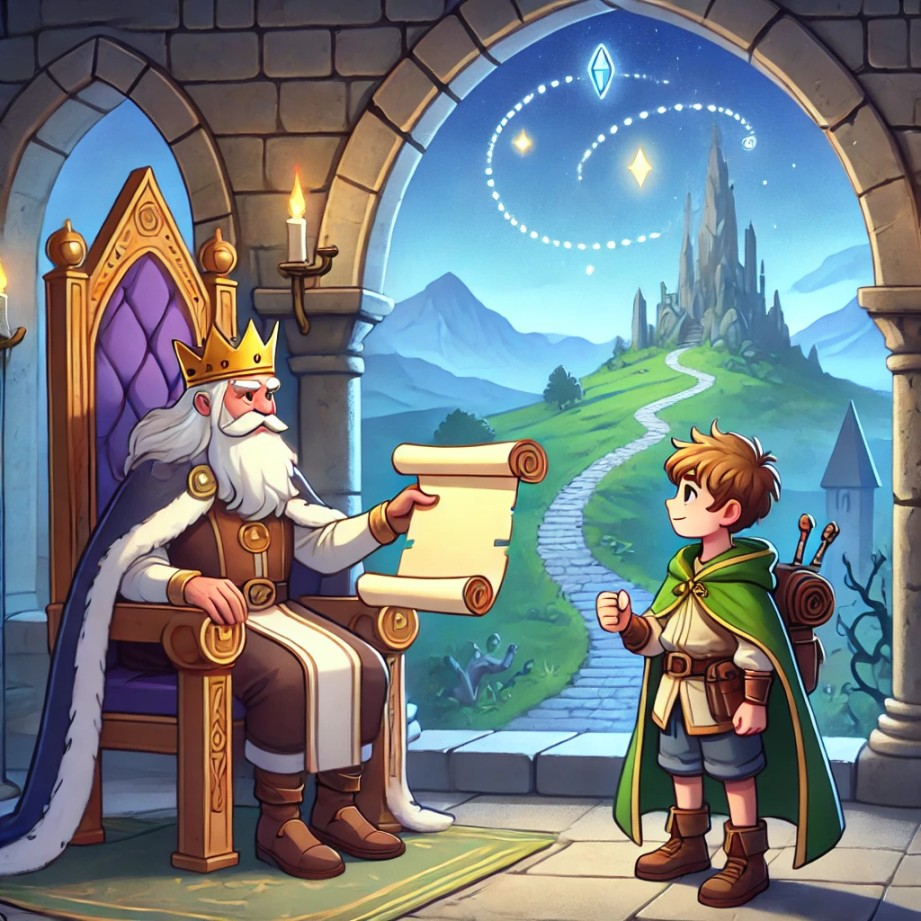
\includegraphics[width=6cm]{scroll.jpg} \\
  \small{The King hands you the magical scroll}
\end{center}

Your mission is to navigate this mysterious path efficiently. Starting from a given scroll, you must determine the smallest number that is greater than or equal to $x$. If no such number exists, you must return to the king with the news that the quest has failed.

\textbf{The Path:}
\begin{itemize}
    \item The path consists of $n$ scrolls, each containing a number and a clue (an index) pointing to the next scroll.
    \item You begin your quest at a scroll indexed as \texttt{start}.
    \item The scrolls are sorted in ascending order, meaning the number on each scroll is less than the number on the next scroll, as long as it exists.
\end{itemize}

\textbf{Your Tools:}
\begin{itemize}
    \item You can ask about a specific scroll by its index to reveal the number it holds and the index of the next scroll.
    \item However, the ancient magic of the path only allows you to ask up to 5000 questions before the path dissolves.
\end{itemize}

You task is to find and report the smallest number on the path that is greater than or equal to $x$. If no such number exists, report that the quest has failed.